\documentclass{article}
\usepackage[utf8]{inputenc}
\usepackage[spanish]{babel}
\usepackage{amsmath}
\usepackage{amsfonts}
\usepackage{amssymb}
\usepackage{lipsum}
\usepackage{xstring} % Paquete necesario para cargar condicionales en newcommand
\usepackage{graphicx} % Paquete necesario que nos permite trabajar con imágenes
\usepackage{vmargin} % Definir los margenes del documento
\usepackage{wrapfig}

\setpapersize{A4}
\setmargins{2.5cm} % margen izquierdo
{1.5cm} % margen superior
{16.5cm} % ancho del area de impresion
{23.42cm} % longitud del area de impresion
{0pt} % espacio para el encabezado
{5mm} % espacio entre el encabezado y el texto
{0pt} % espacio para el pie de pagina
{5mm} % espacio entre el texto y el pie de pagina

% Importar paleta de colores
%archivo paletaColores.tex
\usepackage{xcolor} % Importar el paquete xcolor

% Definir mi paleta de colores
\definecolor{myGreen}{HTML}{36A736}
\definecolor{myBlue}{HTML}{02528F}
\definecolor{blue254}{HTML}{02528F}
\definecolor{myOrange}{HTML}{FF4312}

\title{Ejemplo de uso de Imágenes y Texto en \LaTeX}
\author{Juan Diego Poccori Escalante}
\date{\today}

\begin{document}
    \maketitle
    \renewcommand{\contentsname}{Tabla de contenido}
    \renewcommand{\listfigurename}{Lista de Figuras}
    \renewcommand{\figurename}{Fig.}
    \tableofcontents
    \listoffigures

    \section{Utilizar el ambiente \texttt{wrapfigure}}
    \begin{wrapfigure}[10]{L}[5mm]{.45\textwidth}
        \centering
        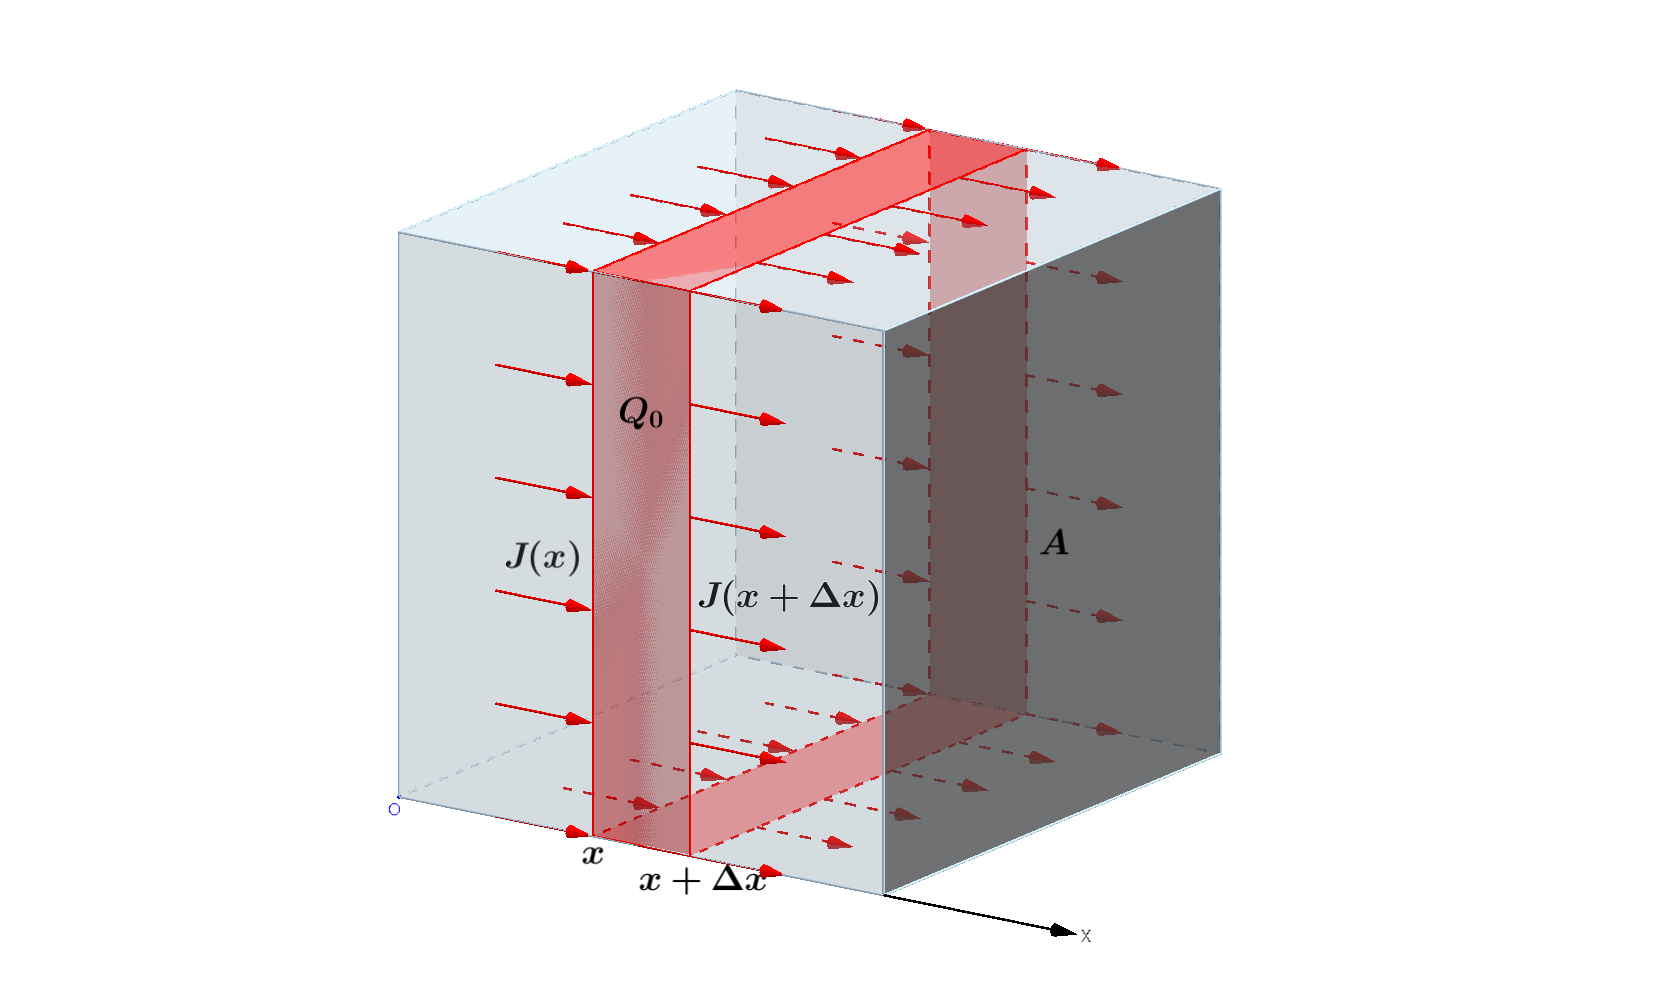
\includegraphics[scale=0.5]{cubo}

    \end{wrapfigure}

    \end{document}
